\chapter{Introduzione}
Con la sindrome del \textit{Blue Baby} ci riferiamo ad un insieme variegato di condizioni anomale e a volte patologiche che si manifestano con la colorazione cianotica della pelle di un neonato.
L'obiettivo principale dei medici è quello di trovare quale tra le patologie che possono portare al colorito blu della pelle sia presente nel bambino, al fine di intervenire repentinamente e in modo mirato sulle cause. Per fare ciò, i medici hanno a disposizioni una serie di esami clinici da compiere, che permettono di rilevare i sintomi tipici di alcune malattie che sono anche causa della sindrome in questione. Analizzando i risultati di questi test, gli specialisti sono in grado di restringere le possibili malattie che affliggono il neonato, individuando così la causa più probabile del colorito anomalo della pelle.

Nel nostro caso, alcuni ricercatori hanno lavorato a stretto contatto con medici ed esperti e sono riusciti a produrre una rappresentazione delle rete di dipendenza delle malattie che causano il fenomeno (Spiegelhalter \textit{et al.}, Statistical science 1993). La rete prodotta, riportata in Figura \ref{fig:paperstructure}, contiene una serie di sintomi, esami e dati sul paziente (\textit{i.e.}, sintomatologia e relativa presentazione) che permettono di modificare la probabilità che una malattia sia presente nell'infante. Tale modello assume che non coesista più di una patologia in ogni paziente che causi la sindrome studiata. Nella rappresentazione proposta è visibile come i nodi della rete si dispongano secondo una struttura ad albero; in particolare, i figli del nodo \textit{Disease} sono situazioni patologiche manifestate in alcune delle malattie che possono causare la sindrome in analisi. I figli di questi nodi sono o nuove situazioni patologiche causalmente collegate alle precedenti, o esami che permettono di accertarne la presenza (\textit{e.g.}, il mescolamento del sangue a livello cardiaco, rappresentata dal nodo \textit{CardiacMixing}, causa un'ipossia polmonare, rappresentata dal nodo \textit{HypoxiaInO2}, che è un figlio del nodo precedente).
 
 \begin{figure}
 	\centering
 	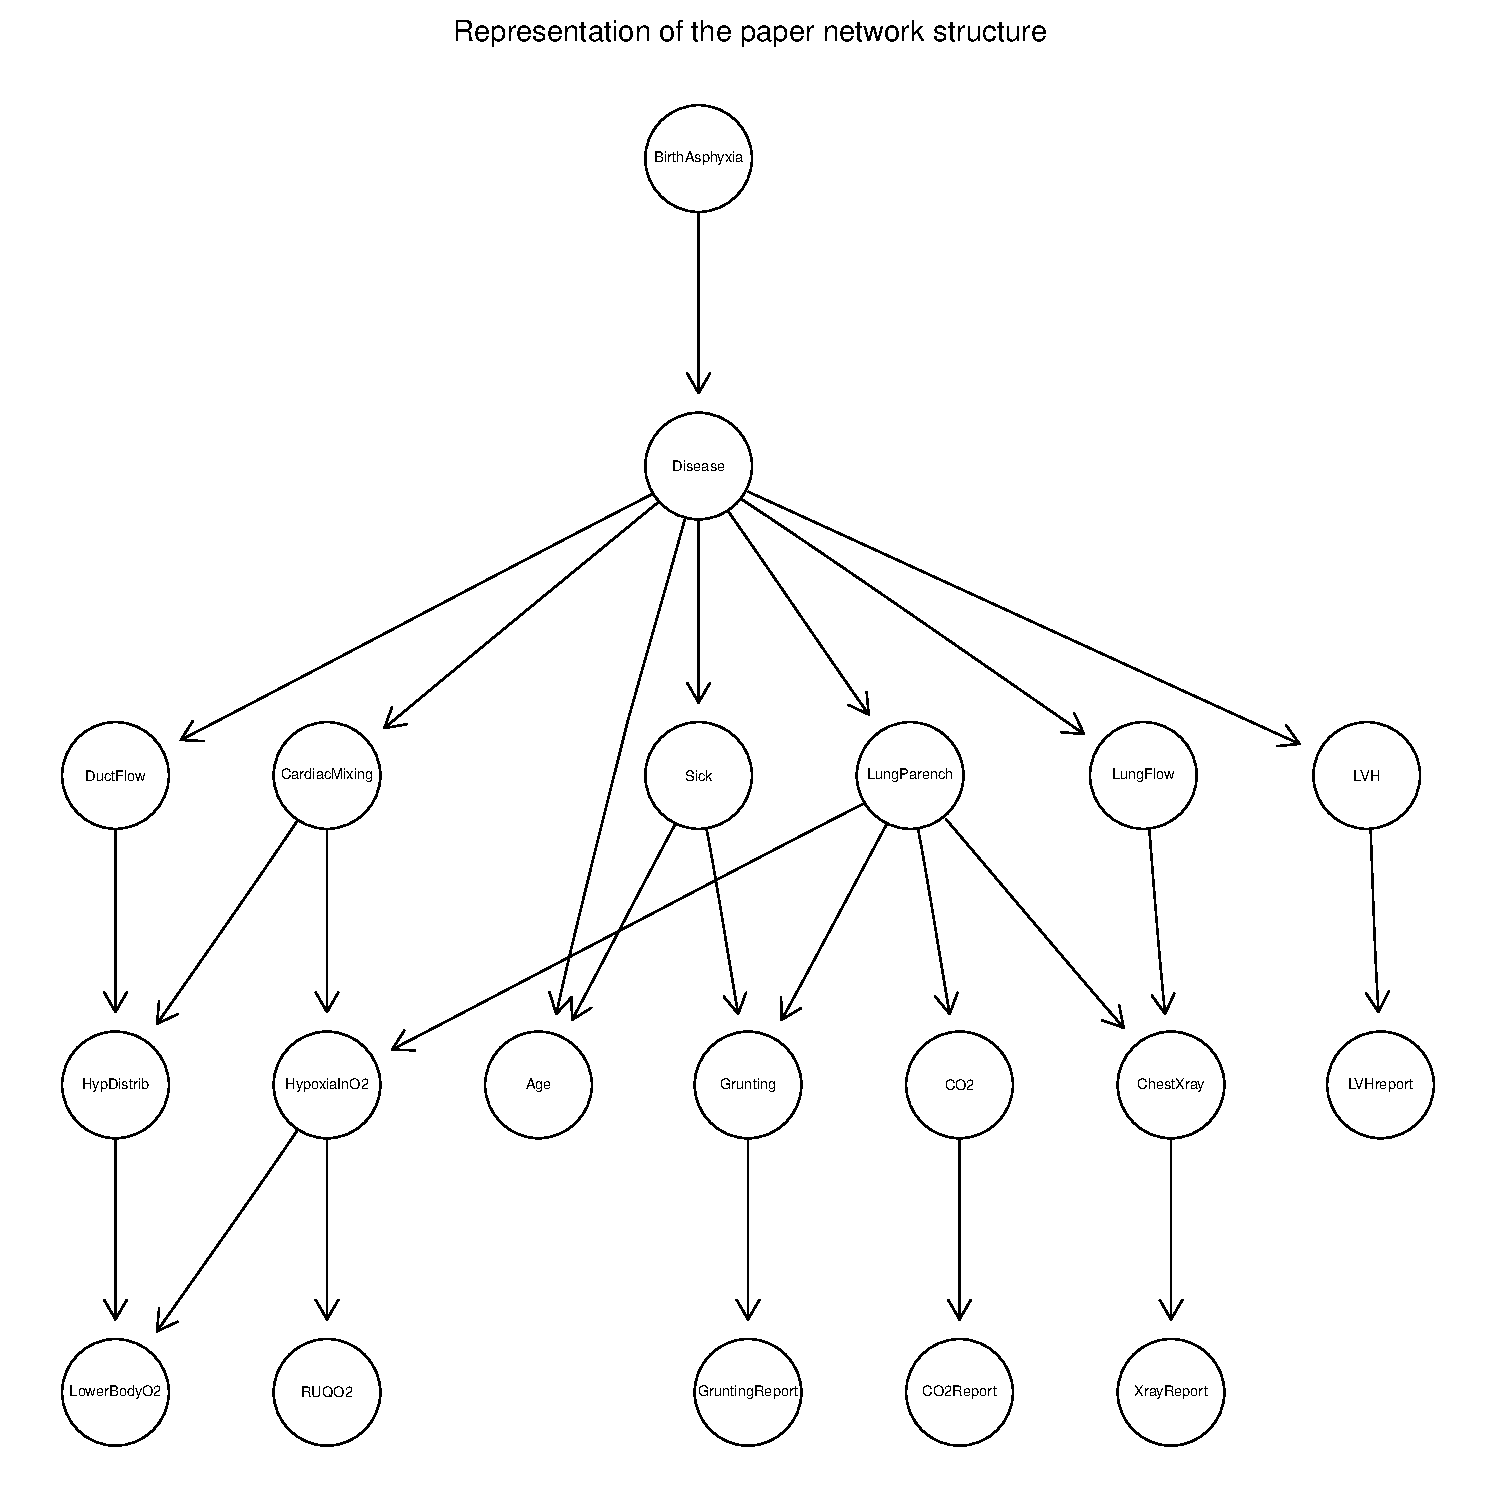
\includegraphics[width=1\linewidth]{images/paper_structure}
 	\caption{Rappresentazione della rete prodotta dai ricercatori, in collaborazione con medici ed esperti. Ogni nodo rappresenta un sintomo, un esame o un dato del paziente.}
 	\label{fig:paperstructure}
 \end{figure}

\section{Obiettivi}
Nel nostro lavoro, abbiamo voluto studiare se fosse possibile inferire la struttura della rete a partire da un dataset contenete evidenze dei nodi della rete in casi accertati della sindrome del \textit{Blue Baby}. Cercheremo poi di capire se vi siano dei nodi che sono condizionalmente indipendenti da altri nodi data l'evidenza di un insieme di variabili, in modo da consentire la riduzione del numero di esami necessari al fine di ottenere una diagnosi accurata. Vaglieremo inoltre la possibilità di utilizzare la rete invertendo le relazioni di causalità, analizzando i risultati ottenuti e comparandoli quelli della rete proposta. Ci siamo infine posti l'obiettivo di produrre un'interfaccia grafica nella quale il medico sia in grado di inserire il valore dei nodi di cui ha conoscenza e ottenere una stima della probabilità della presenza delle varie malattie nel neonato.